\subsection{Minh họa giao diện, sơ đồ hoạt động hoặc prototype đơn giản.}

Các hình dưới đây minh họa prototype MVP của \textbf{1Stream} theo ba nhóm chức năng chính: luồng tạo nội dung AI, trợ lý bán hàng trong phiên live và khu vực cấu hình/quản trị hệ thống. Cách trình bày theo nhóm giúp làm rõ vai trò của từng màn hình trong quy trình vận hành tổng thể, thay vì chỉ liệt kê các ảnh giao diện rời rạc.

\subsubsection*{Nhóm 1: Luồng AI cốt lõi của MVP}

\begin{figure}[H]
    \centering
    \begin{minipage}[t]{0.48\textwidth}
        \centering
        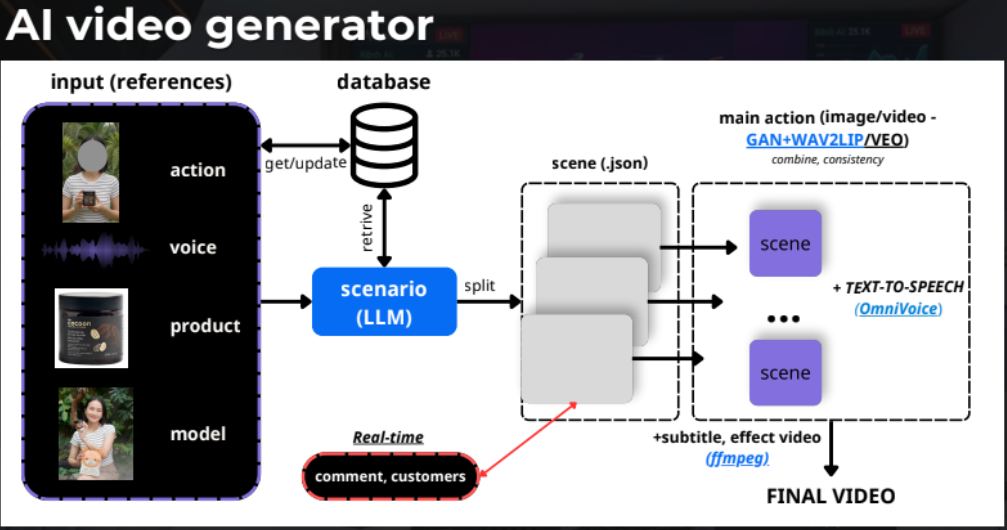
\includegraphics[width=\linewidth]{imgs/mvp1.png}
        \vspace{3pt}

        \textbf{AI Video Generator}\\
        {\small Sơ đồ tạo video livestream từ dữ liệu đầu vào như hành động mẫu, giọng nói, sản phẩm và nhân vật mẫu. Hệ thống dùng LLM để tách kịch bản thành từng cảnh, sau đó kết hợp tạo hình ảnh/video, text-to-speech và hậu kỳ để xuất video hoàn chỉnh.}
    \end{minipage}
    \hfill
    \begin{minipage}[t]{0.48\textwidth}
        \centering
        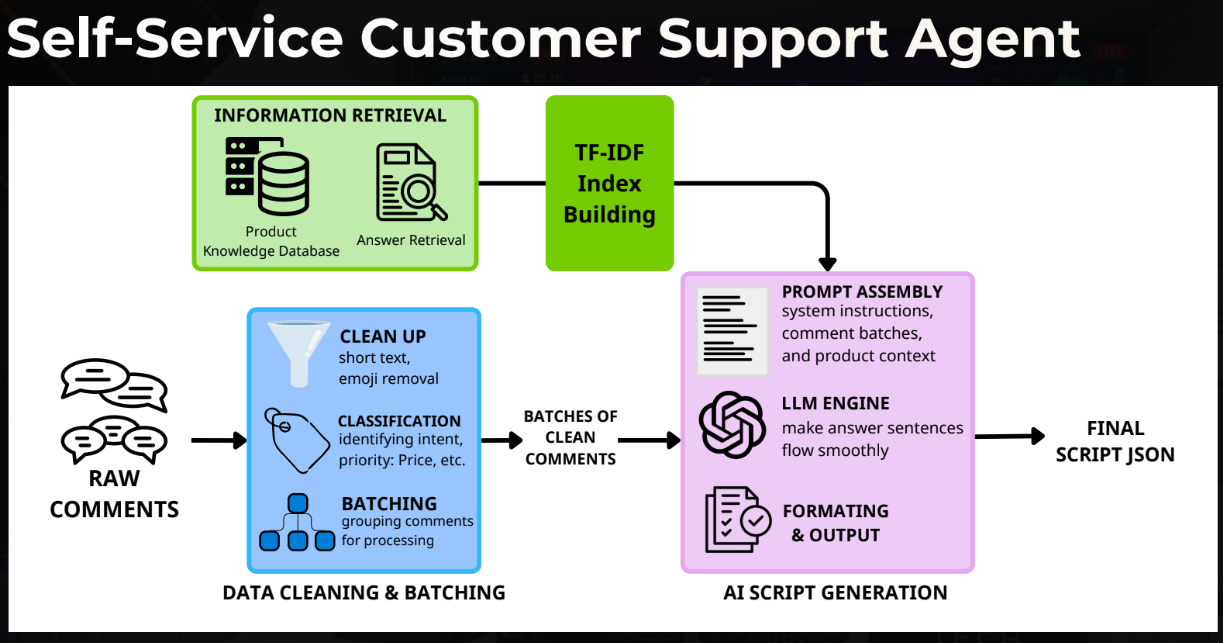
\includegraphics[width=\linewidth]{imgs/mvp2.png}
        \vspace{3pt}

        \textbf{Self-Service Customer Support Agent}\\
        {\small Sơ đồ xử lý bình luận khách hàng: làm sạch dữ liệu, phân loại ý định, gom nhóm bình luận, truy xuất thông tin sản phẩm bằng TF-IDF và dùng LLM để tạo câu trả lời phù hợp ngữ cảnh.}
    \end{minipage}
    \caption{Hai luồng AI nền tảng của MVP: tạo nội dung livestream và phản hồi khách hàng tự động}
    \label{fig:mvp-core-ai-flows}
\end{figure}

\subsubsection*{Nhóm 2: Giao diện vận hành phiên livestream}

\begin{figure}[H]
    \centering
    \begin{minipage}[t]{0.48\textwidth}
        \centering
        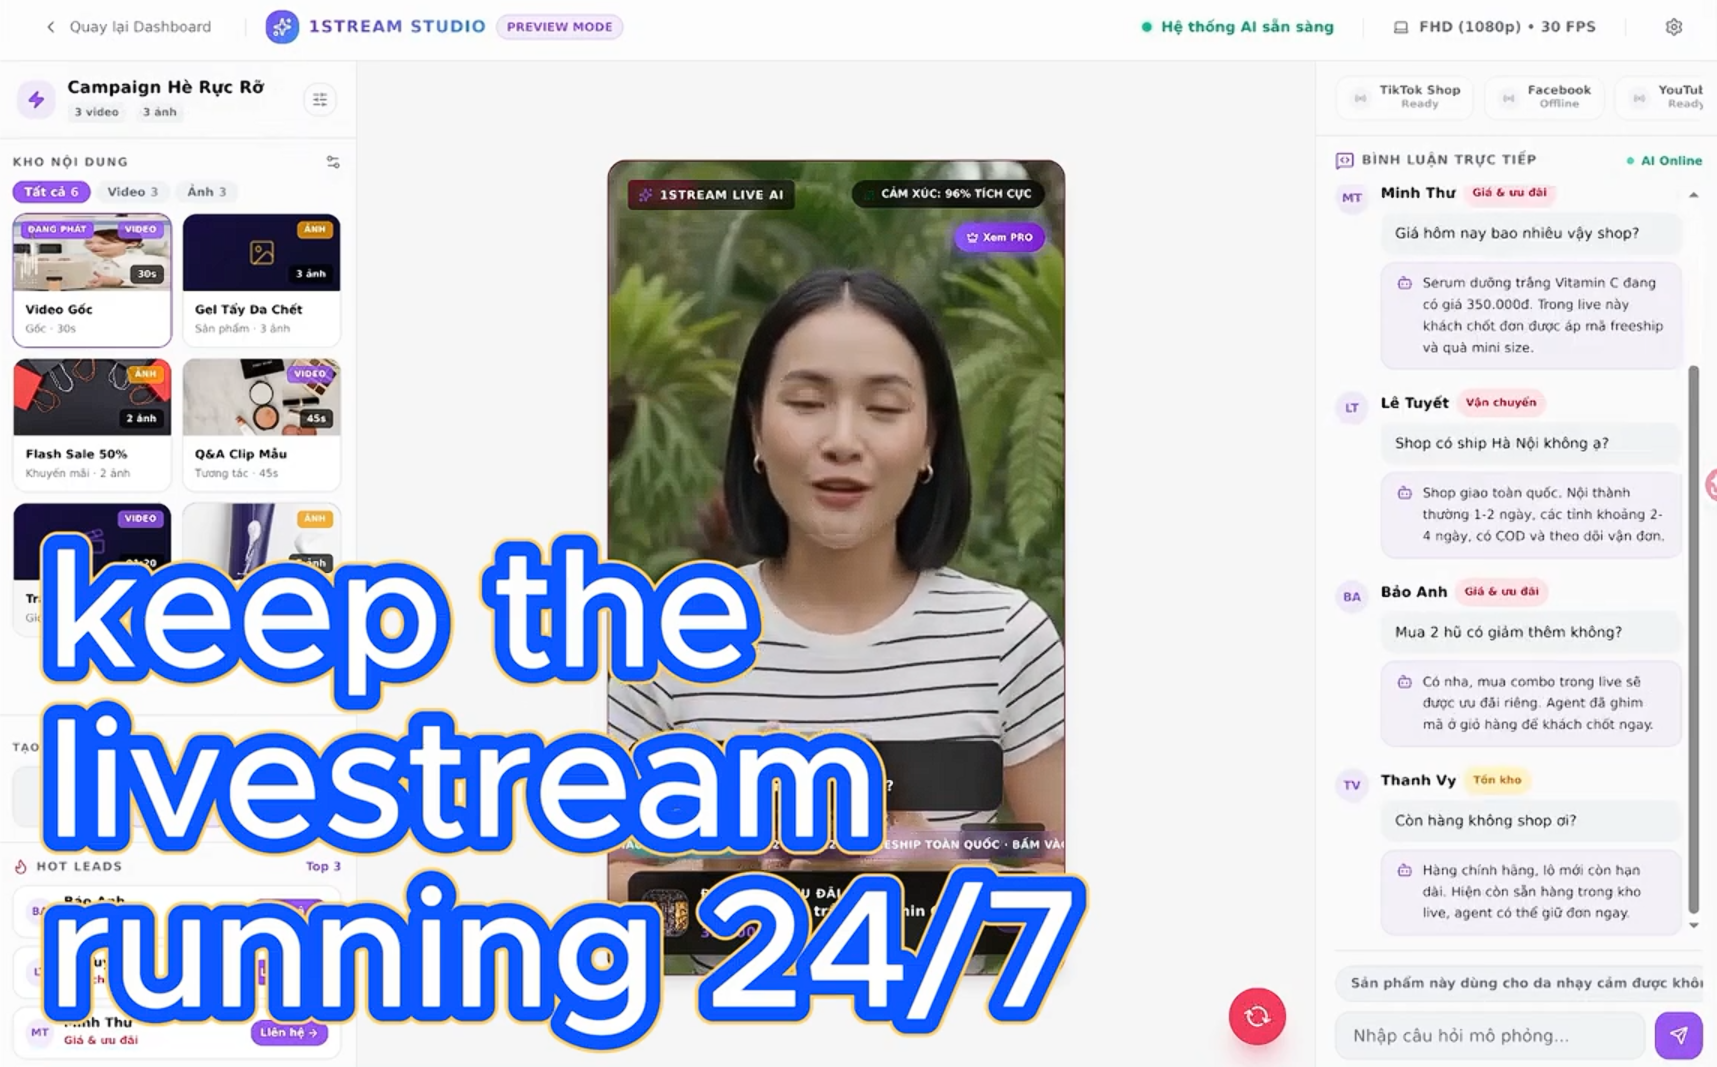
\includegraphics[width=\linewidth]{imgs/mvp3.png}
        \vspace{3pt}

        \textbf{Live Studio Preview}\\
        {\small Màn hình studio cho phép người bán theo dõi video đang phát, quản lý thư viện nội dung, xem trạng thái kênh livestream và quan sát bình luận trực tiếp cùng phản hồi do AI đề xuất.}
    \end{minipage}
    \hfill
    \begin{minipage}[t]{0.48\textwidth}
        \centering
        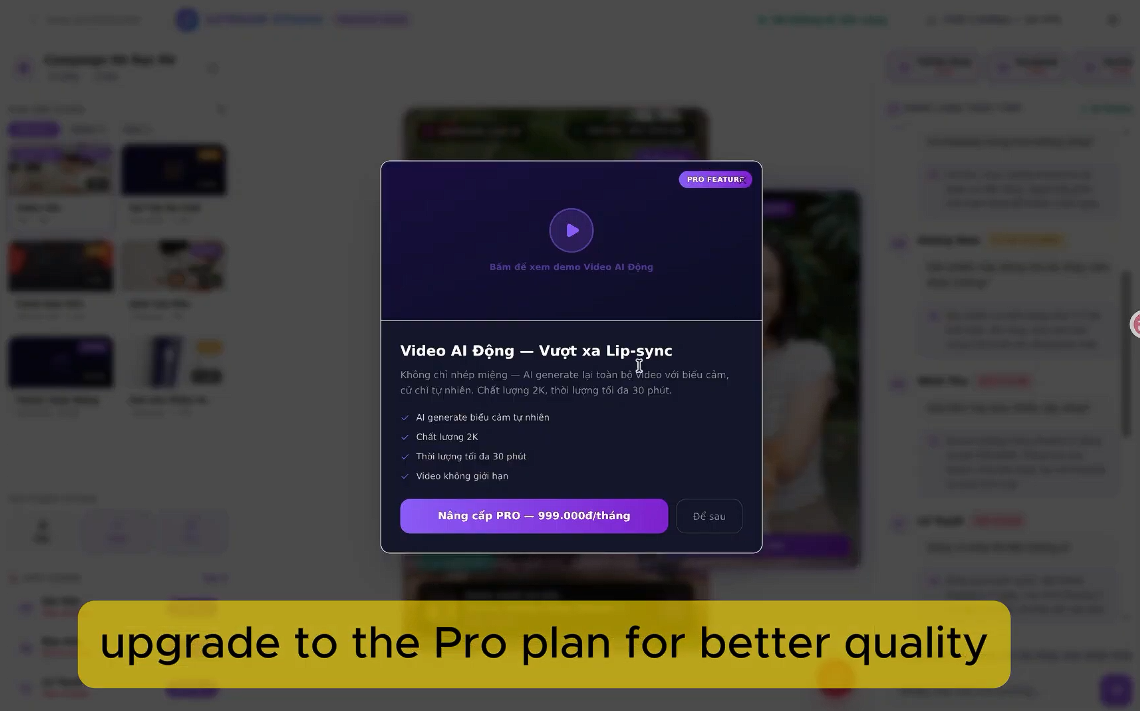
\includegraphics[width=\linewidth]{imgs/mvp4.png}
        \vspace{3pt}

        \textbf{Dynamic AI Video Upgrade}\\
        {\small Màn hình giới thiệu tính năng video AI động thuộc gói Pro, cho thấy định hướng thương mại hóa theo cấp độ chất lượng video, thời lượng tạo nội dung và khả năng tạo biểu cảm tự nhiên.}
    \end{minipage}
    \caption{Giao diện vận hành livestream và phân tầng tính năng nâng cao trong MVP}
    \label{fig:mvp-live-operation}
\end{figure}

\subsubsection*{Nhóm 3: Cấu hình, quản trị và cập nhật dữ liệu}

\begin{figure}[H]
    \centering
    \begin{minipage}[t]{0.48\textwidth}
        \centering
        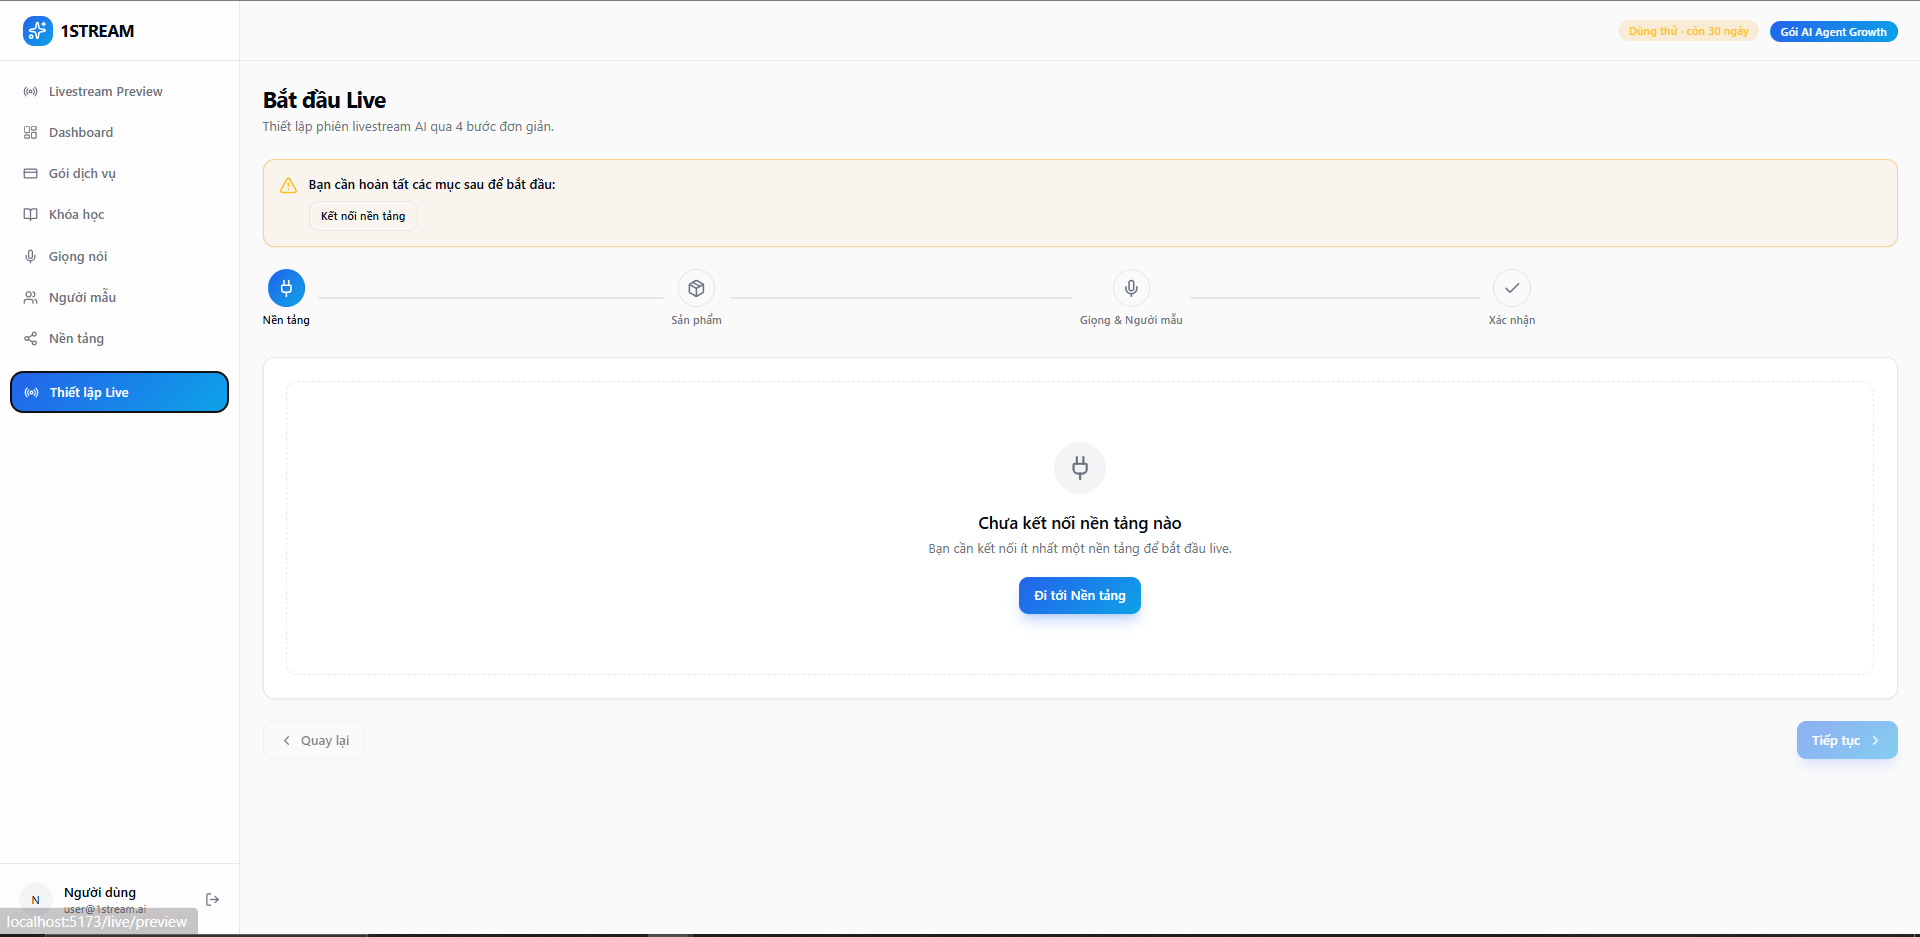
\includegraphics[width=\linewidth]{imgs/mvp5.png}
        \vspace{3pt}

        \textbf{Live Setup \& Content Library}\\
        {\small Khu vực thiết lập phiên live, chọn video lip-sync, phát live loop, tạo thêm video AI mới và theo dõi bình luận trong cùng một không gian vận hành.}
    \end{minipage}
    \hfill
    \begin{minipage}[t]{0.48\textwidth}
        \centering
        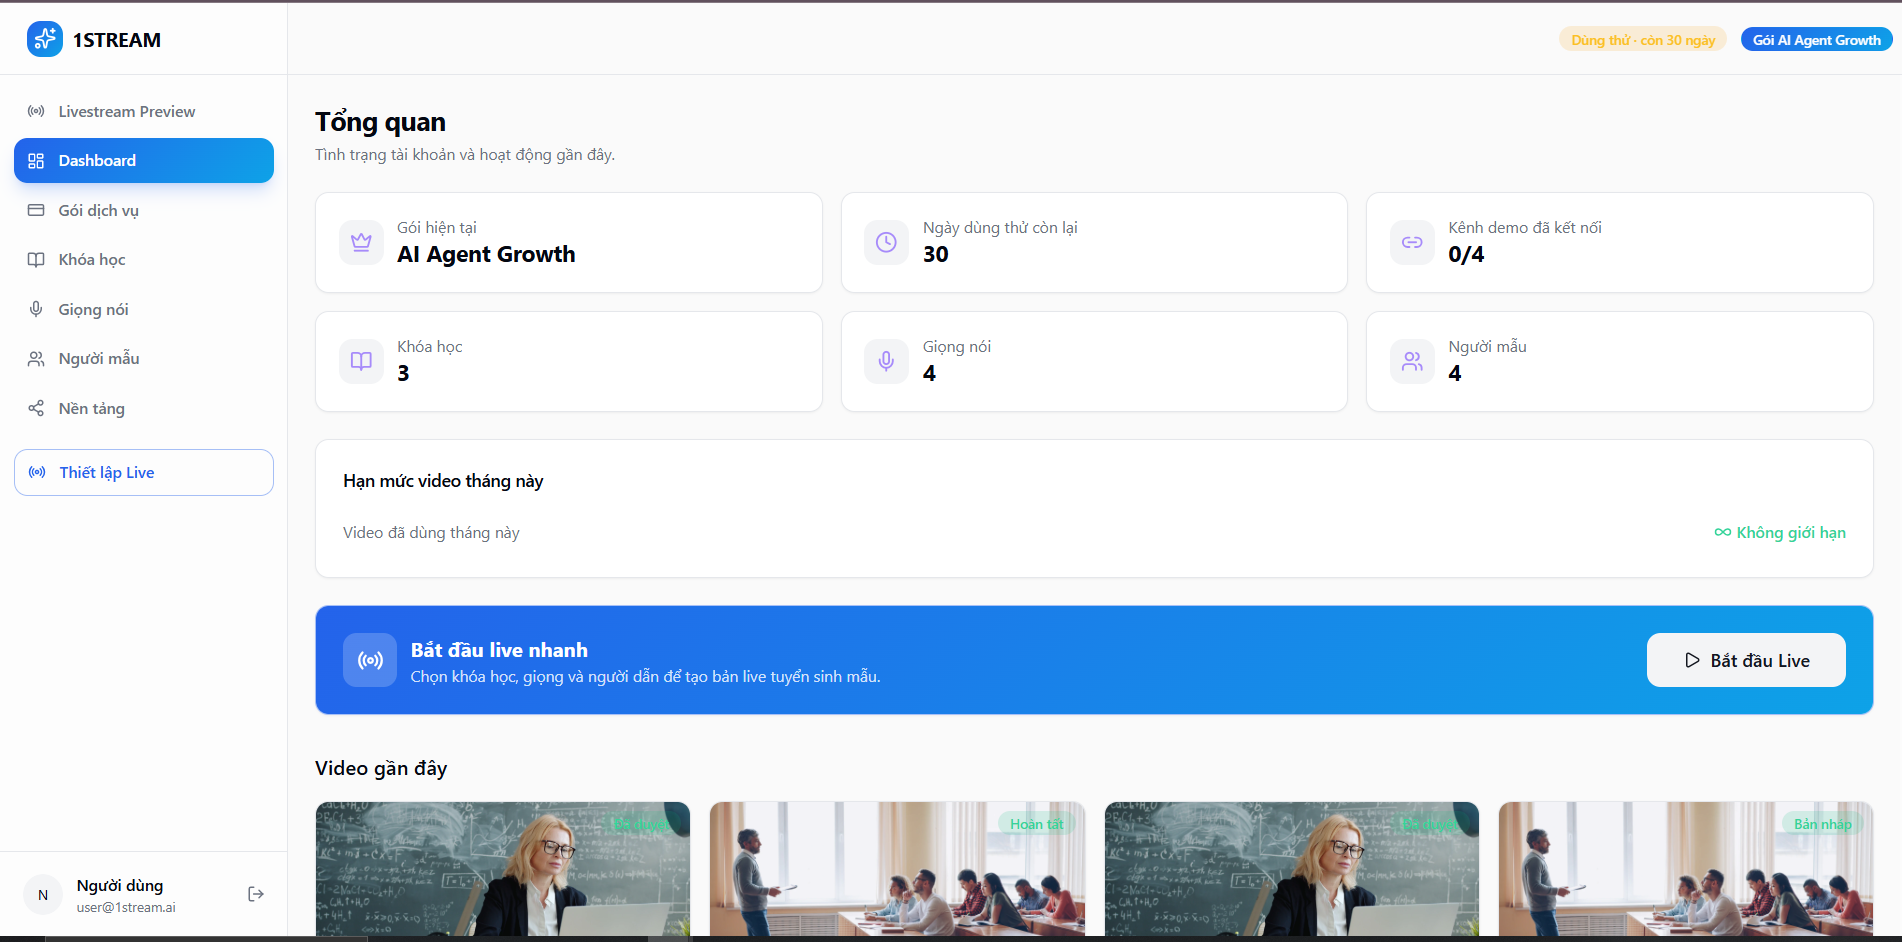
\includegraphics[width=\linewidth]{imgs/mvp6.png}
        \vspace{3pt}

        \textbf{Dashboard \& System Configuration}\\
        {\small Dashboard tổng quan cho phép người bán theo dõi gói dịch vụ, số sản phẩm, giọng nói, người mẫu, nền tảng đã kết nối và truy cập nhanh vào quy trình bắt đầu phiên live.}
    \end{minipage}
    \caption{Nhóm màn hình cấu hình, quản trị dữ liệu và chuẩn bị phiên livestream}
    \label{fig:mvp-config-dashboard}
\end{figure}
